%mainfile: rapport.tex

\section{Algorithme réparti}

\lstinputlisting[caption={Algorithme réparti}]{algo.txt}

\subsection{Explication de l'algorithme}
\subsubsection{Initialisation}
Lors du démarrage de l'application, la base de données est reconstruite. Celle-ci comporte trois stockages, plus une vue :
\begin{description}
	\item[bd\_abos] contient l'ensemble des identifiants de n\oe uds, et pseudos d'utilisateurs auxquels le n\oe ud courant est abonné.
	\item[bd\_offres\_abo] contient l'ensemble des identifiants de n\oe uds, ainsi que la distance des abonnements offerts à portée. Cette liste comporte des priorités, permettant de détruire les abonnements passagers dus à un simple croisement avec un véhicule.
	\item[bd\_demandes\_abo] a un fonctionnement identique à la base d'offres. Cependant, elle intègre une partie des abonnements désirés par les voisins.
	\item[bd\_flux] correspond à une vue des publications issues du n\oe ud courant et de ses abonnés. Elle correspond au flux qui sera visualisé par l'utilisateur final.
\end{description}
\paragraph*{}
Un timer est ensuite enclenché afin d'effectuer à intervalle régulier un \msgheartbeat.

\subsubsection{\heartbeat}
Ce message correspond à un battement de c\oe ur, c'est à dire, une preuve d'existence. Il est diffusé à tous, mais ne pourra être relayé. Son contenu (offres et demandes du n\oe ud et de ses voisins environnants) servira à mettre à jour les bases de données des n\oe uds receveurs. Ce contenu pourra alors très bien figurer dans les messages \msgheartbeat\ des n\oe uds receveurs. Ce système permet de répartir la base de donnée générale des \textit{abonnements - abonnés} et ceci même lorsqu'aucun message \pie\ n'est transmis.

\paragraph*{}
Afin de former ce message, il faut tout d'abord nettoyer les bases de données. La priorité de chaque offre et demande va être décrémentée, afin que les n\oe uds que nous ne rencontrons plus aient une priorité négative. Cette priorité pourra être calculée, uniquement sur le nombre de messages \msgheartbeat\ de la cible, ou en prenant en compte les coordonnées GPS de celle-ci. Au contraire, à la réception d'un message, les abonnements contenus dans les offres et les demandes verront leur priorité incrémentée.

\subsubsection{Envoi et réception d'un message \pie}
Un message \pie{} correspond à la publication que l'utilisateur veut envoyer à ses suiveurs, de la même façon que sur \twitter. Ce message doit donc être acheminé jusqu'à chaque voiture concernée par notre abonnement. Insérer une limite de distance dans la diffusion du message impliquerait un rayon de diffusion fixe, et ainsi, un long convoi de véhicules ne sera pas pris en compte. Augmenter la distance maximale de diffusion suppose une diffusion lointaine, probablement vers des zones n'ayant aucun intérêt pour notre abonnement. C'est pour cela que nous avons introduit deux notions : le \fkttl\ et le \fktts.

\paragraph*{}
Le \fkttl\ (Time To Live) va être décrémenté chaque fois qu'un n\oe ud retransmet le message alors que l'abonnement ne figure pas dans sa base de donnée \texttt{bd\_demandes\_abo}.
\paragraph*{}
Le \fktts\ (Time To Survive) va être décrémenté par chaque n\oe ud retransmettant le message alors que l'abonnement figure dans la base de donnée \texttt{bd\_demandes\_abo}.
\paragraph*{}
Un seul de ces deux compteurs peut être décrémenté. Le message n'est pas retransmis si le compteur devant être décrémenté est à 0. Ce mode de retransmission permet une diffusion intelligente. En effet, bien que le message puisse être diffusé inutilement dans un rayon égal au \fkttl, il pourra cependant s'étendre d'avantage dans les zones où un destinataire est présent, grâce au \fktts. Le schéma ci-dessous montre ce principe.

\begin{center}
	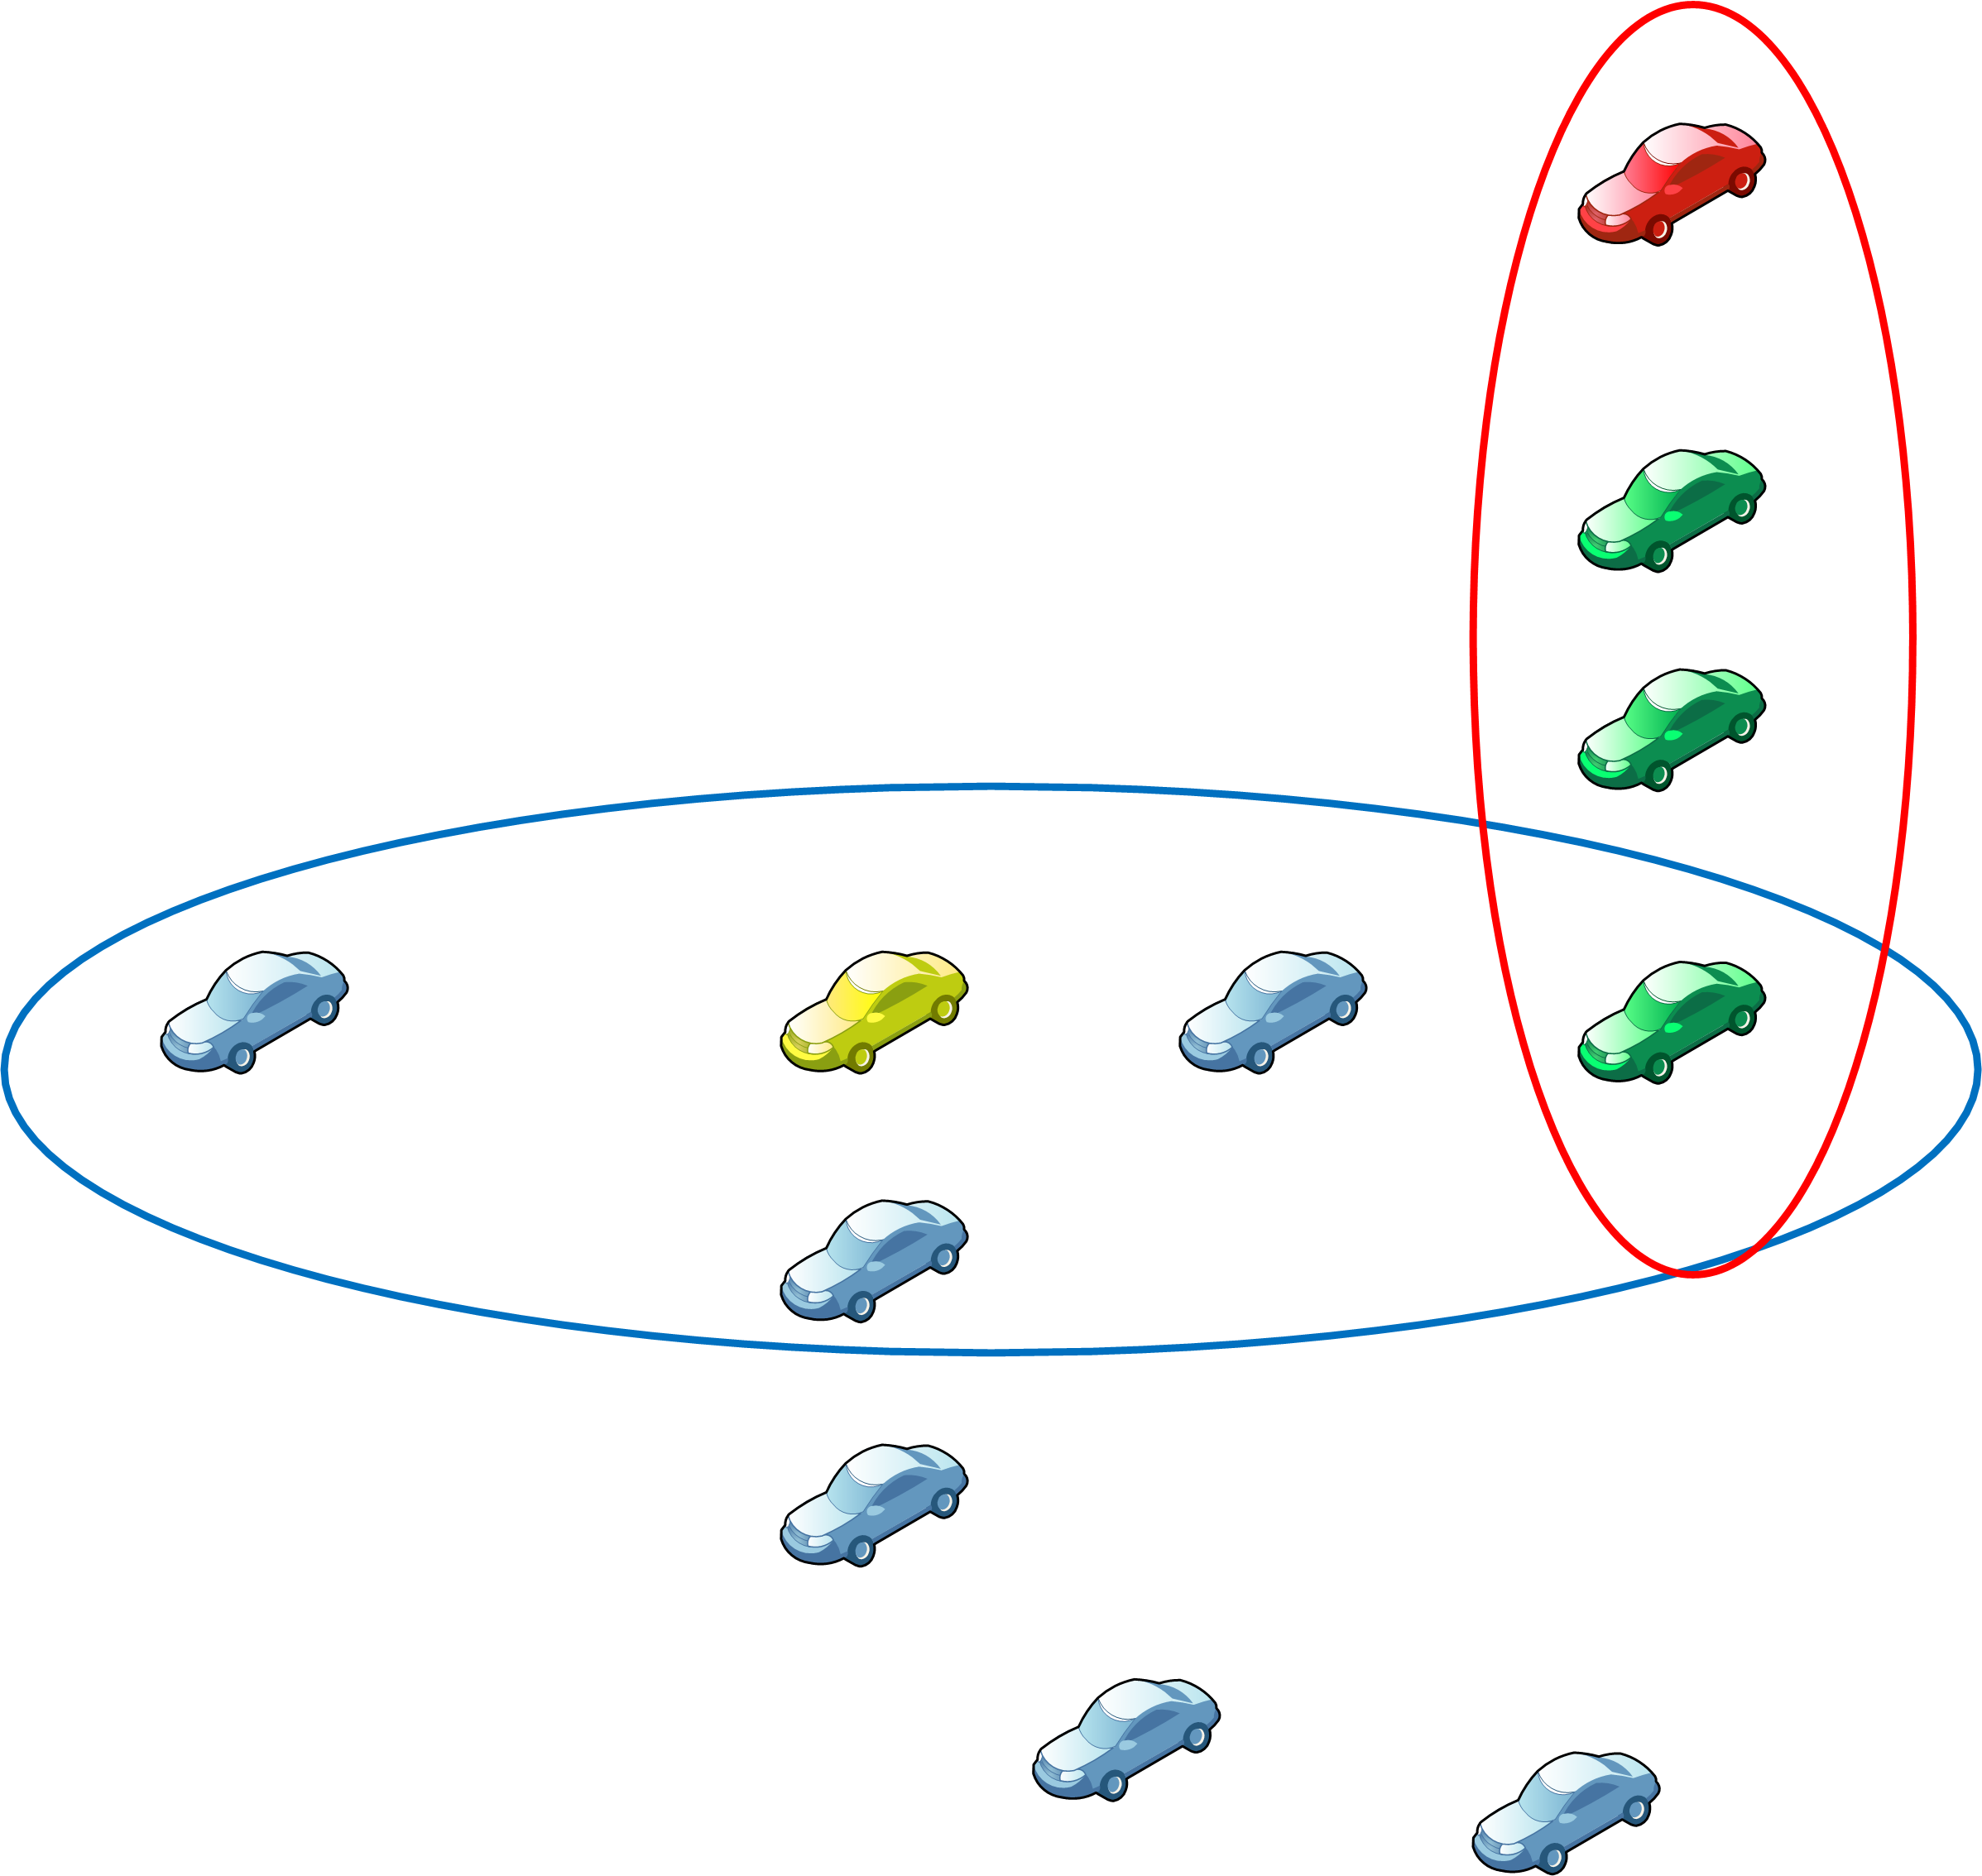
\includegraphics[width=0.75\textwidth]{img/schema2}
\end{center}

\paragraph*{}
\begin{description}
	\item[Voiture jaune :] N\oe ud émetteur du message PIE.
	\item[Voiture bleue :] N\oe ud non abonné et non intéressé par le message.
	\item[Voiture verte :] N\oe ud non abonné, mais connaissant un n\oe ud intéressé par celui-ci.
	\item[Voiture rouge :] N\oe ud abonné à l'émetteur désirant donc recevoir le message.
	\item[Ellipse bleue :] Zone de diffusion du message par décrémentation du \fkttl.
	\item[Ellipse rouge :] Zone de diffusion du message par décrémentation du \fktts.
\end{description}
\paragraph*{}
Nous remarquons que contrairement à une diffusion par distance qui aurait un format de cercle, l'utilisation du \fkttl\ et \fktts\ permet une diffusion ayant une forme variable. Dans le cas d'un convoi de véhicules, avec un véhicule égaré, cela va par exemple permettre de continuer à faire communiquer les deux protagonistes le plus longtemps possible.


\paragraph*{}
% Jérémy: pas d'ac, on en rediscute ;)
Dans un soucis d'optimiser chaque message, et d'avoir une convergence rapide entre les bases de données et la topologie physique de notre réseau de voitures, nous avons choisi d'inclure les offres et les demandes aux messages \pie. Ainsi, ces messages participeront à un meilleur acheminement des futurs messages du réseau. Le réseau étant dynamique, les routes seront constamment réévaluées.

